\documentclass[paper-main.tex]{subfiles}

\begin{document}


% Optical microphone
% aim of optical microphone: play back injected sounds
% some editing in response to pnp
In this section we explore how this demonstration can be used to teach a selection of signal processing techniques.
The apparatus used in Sections~\ref{sec:ifo} to~\ref{sec:viterbi_wandering} affords the opportunity to explore a range of signal processing techniques and filters of interest to undergraduate students and provide a foundations for many technical applications~\cite{DigitalProcingOfSpeechSignals:1978}. 
We provide a series of example activities using complex audio (such as music and speech) as a natural successor to constant and wandering tones. 
%A natural successor to constant and wandering tones is complex audio, such as music and speech. 
As complex audio signals are not quasi-monochromatic, unlike continuous gravitational wave signals, the Viterbi algorithm as implemented in Section~\ref{sec:viterbi_wandering} is not directly applicable here. Instead, in this section, we use the interferometer as an \emph{optical microphone} to detect and play back complex audio signals (i.e.\ using light to capture sound).
In doing so, we experiment with a hierarchy of passive filters which suppress noise yet make no assumption about the specific form of the signal, unlike the Fourier-based maximum likelihood matched filter which is tuned to the sinusoidal signals in Section~\ref{sec:single_tone} and Appendix~\ref{app:sinusoid_likelihood}.
A vast literature exists on signal processing with speech, however see Ref.~\cite{DigitalProcingOfSpeechSignals:1978} for introductory material including Fourier analysis and digital representations.
Optical microphone devices have precedence in the laser microphones~\cite{laser_microphone} which are (or were historically) used in the defence industry and operate on a variety of related principles.
  
%An introduction to ..... can be found in Ref.~\cite{}, including 
%A review of digital processing techniques for speech signals can be found 
%It is also analogous to the detection of unmodelled gravitational-wave signals, e.g. broadband bursts from supernovae~\cite{}\han{to do - add citation}. 
%It is also analogous to the detection of unmodelled gravitational wave signals, e.g. broadband bursts from supernovae. [refs; my last sentence can be improved]


This section is indirectly related to the advanced signal processing techniques required to extract gravitational-wave signals.
Here, the optical microphone serves as an independent demonstration for a broader physics and engineering audience, particularly in undergraduate laboratories.
We describe the additional hardware components required for this demonstration in Section~\ref{sec:photodiode} and initial results in Section~\ref{sec:initialResultsOpMic}. 
A selection of filter and speech enhancement example activities using the optical microphone are outlined in Section~\ref{sec:filters}.



\subsection{Hardware modifications for the optical microphone}
\label{sec:photodiode}
% advanced method: explain how we capture data


Audible frequencies are in the range of $\sim 20\,{\rm Hz}$--$20\,{\rm kHz}$. Speech intelligibility requires frequencies up to $3\,{\rm kHz}$ and music requires up to and beyond $8\,{\rm kHz}$~\cite{speech_intelligibility}. Therefore the optical microphone requires a sample rate of at least $16\,{\rm kHz}$ to capture both speech and music. This cannot be achieved with the webcam used in Sections~\ref{sec:single_tone} and ~\ref{sec:viterbi_wandering} as it has a sampling rate of $30\,{\rm Hz}$.
To overcome this issue, we use a photodiode\footnote{A photodiode is an electrical component that acts as a regular diode when no light is incident on it, blocking any current flow in the reverse direction. As the intensity of incident light rises, it becomes increasingly conductive in the reverse direction.} at the output of the interferometer to achieve a sampling rate of $16\,{\rm kHz}$.

We place a OSRAM BPW21 photodiode in reverse-bias over an LM358 op-amp which together make a photo-detector that produces a voltage dependent on the incident intensity. 
The photodiode records the interference pattern at roughly the same off-centre position as the webcam in Sections~\ref{sec:single_tone} and~\ref{sec:viterbi_wandering}, again chosen arbitrarily.
The photodiode is mounted on a cloth screen re-purposed from the dismantled commercial speaker, with the electrical leads connected underneath. 
The voltage signal from the photo-detector is captured by a MCP3008 $10$-bit analog-to-digital converter (ADC) connected to a Raspberry Pi (Pi) Model 3 v1.2~\cite{RaspberryPi:online}, which provides a convenient means to record the photodiode data.
Together, the circuit samples the signal at $\sim 16\,{\rm kHz}$. Resources for using the Pi and photodiode are described in Appendix~\ref{app:circuit_diagram}.

Sampling any frequency component of the analog signal above the Nyquist frequency of $8\,{\rm kHz}$ leads to aliasing\footnote{Folding of frequencies greater than half the sampling rate.} into the detected range. We include an anti-aliasing Sallen-Key filter~\cite{sallen_key_filter} tuned to $16\,{\rm kHz}$ before the ADC to prevent this from happening.
This component attenuates any frequencies above $8\,{\rm kHz}$, before they are digitally sampled. We also place a cloth screen over the face of the photodiode to reduce the intensity of the voltage signal and avoid saturating the ADC.
% It’s not clear what limited the sample rate to 16kHz, but it was likely non-optimal reading of the ADC by the Pi script.
% The ADC used (MCP3008) is quoted at 200kHz (or ksps, kilo samples per second).

An updated schematic is shown in Fig.~\ref{fig:ifo_schematic_podo} and a photograph of the entire optical microphone in Fig.~\ref{fig:setup_pic2}.
See Appendix~\ref{app:circuit_diagram} for a diagram and photograph of the circuit. 


\begin{figure*}
	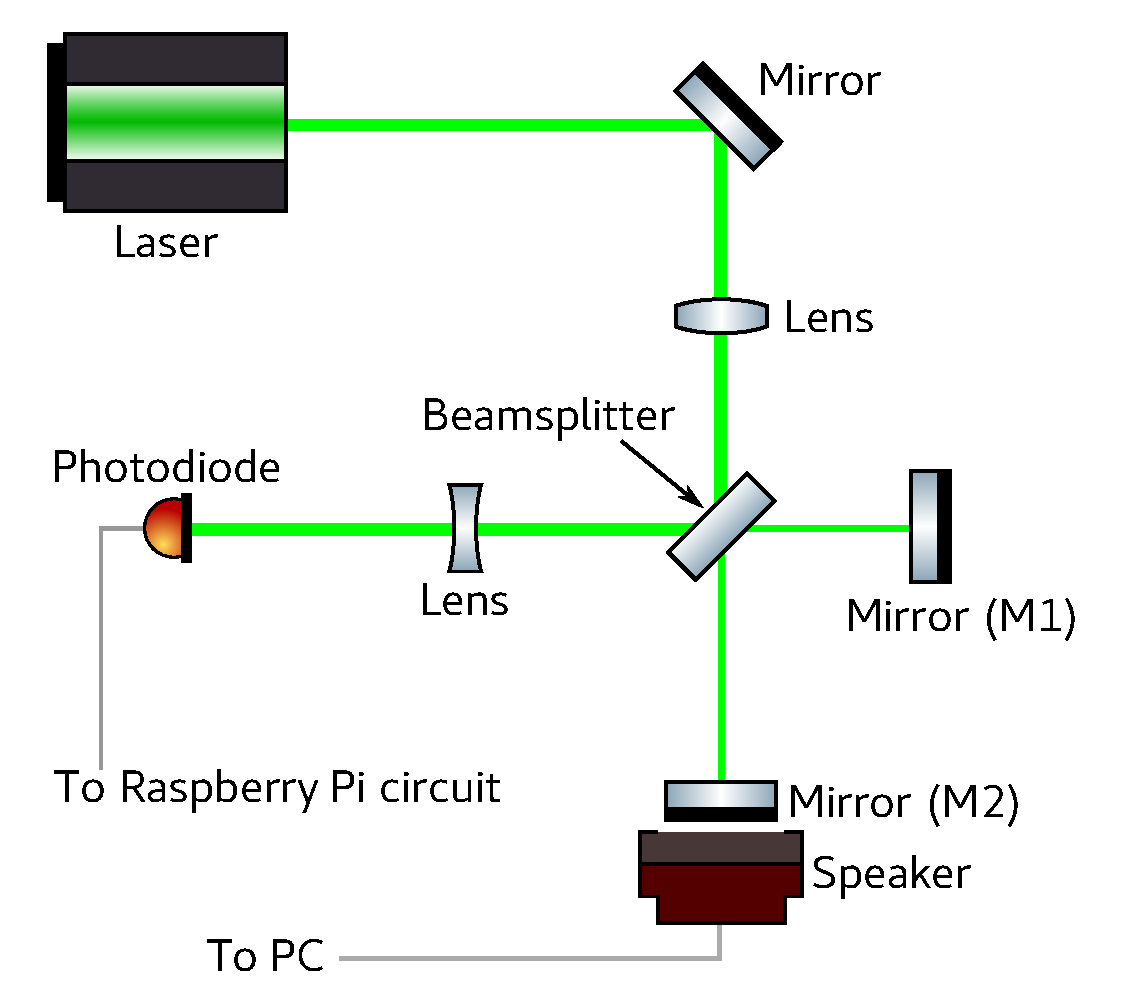
\includegraphics[width=0.44\textwidth]{figures/ifo_schematic_photodiode_edit.pdf}
	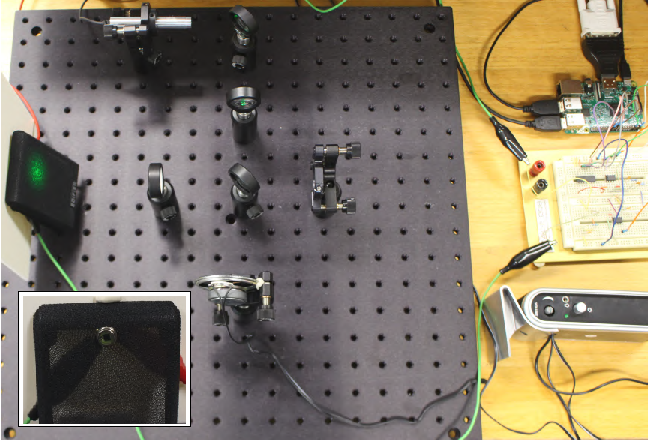
\includegraphics[width=0.52\textwidth]{figures/setup_pic2.pdf}
	\caption{
Left: Michelson interferometer schematic. 
The schematic is identica.l to Figure~\ref{fig:interference_pattern} except that the data is now recorded using a photodiode and Raspberry Pi instead of a webcam. 
Right: photograph of the optical microphone. 
The Michelson interferometer is shown on the left and the circuit and Raspberry Pi on the right. 
In the main image, the photodiode is placed behind the cloth screen. 
The inset shows a face-on view of the photodiode with the covering screen removed. 
See Appendix~\ref{app:circuit_diagram} for a circuit diagram and detailed photograph of the circuit.
}
	\label{fig:ifo_schematic_podo}
\end{figure*}

\begin{comment}
\begin{figure}
	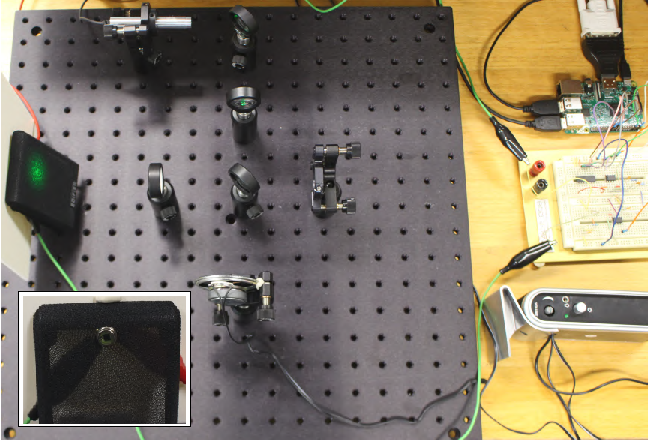
\includegraphics[width=.49\textwidth]{figures/setup_pic2.pdf}
\caption{Photograph of the optical microphone. The Michelson interferometer is shown on the left and the circuit and Raspberry Pi on the right. The interferometer is laid out as in Figure~\ref{fig:ifo_schematic_podo}. In the main image, the photodiode is placed behind the cloth screen. The inset shows a face-on view of the photodiode with the covering screen removed. See Appendix~\ref{app:circuit_diagram} for a circuit diagram and detailed photograph of the circuit.}
	\label{fig:setup_pic2}
\end{figure}
\end{comment}

\subsection{Anti-aliased output}
\label{sec:initialResultsOpMic}

%The source audio was played through the speaker with the optical microphone recording for the full duration of the audio (around a minute long for most sources). 
We test the optical microphone with a variety of recordings including speech from different people and music ranging from simple melodies and rhythms to songs. During recordings, care is taken to minimise activity around the demonstration to reduce the amount of environmental noise coupling into the interferometer. The time series data is then directly converted to a .wav file and played as an audio recording using the \textbf{io.wavfile.write} function. When processing the results, we restrict our analysis to only the first $10\,{\rm s}$ of each observation (for efficiency), and only plot the first second here. 

The raw output of the optical microphone (with anti-aliasing) is noisy with a loud bass hum throughout. This can be explained by looking at the power spectral density (PSD) of the background noise (i.e., with the speaker switched off), as shown in the top panel of Fig.~\ref{fig:psd_noise}. The spectrum is dominated by AC mains noise with power from the fundamental $50\,{\rm Hz}$ mains signal up to and beyond $8$th harmonic thereof. The mains signal is also present (but far weaker) in the background spectrum taken with the photodiode in darkness, suggesting that ambient lighting has a large contribution. Besides lighting, other possible contributions to the mains signal include air conditioning and the photodiode circuit itself. The appearance of harmonics of the mains noise is likely due to the non-linearity discussed in Appendix~\ref{app:intensity_derivation} (see also Ref.~\cite{feynman}). The spectrum in Fig.~\ref{fig:psd_noise} also has a broad feature at around $750\,{\rm Hz}$, the origin of which is yet to be determined.


\begin{figure}
	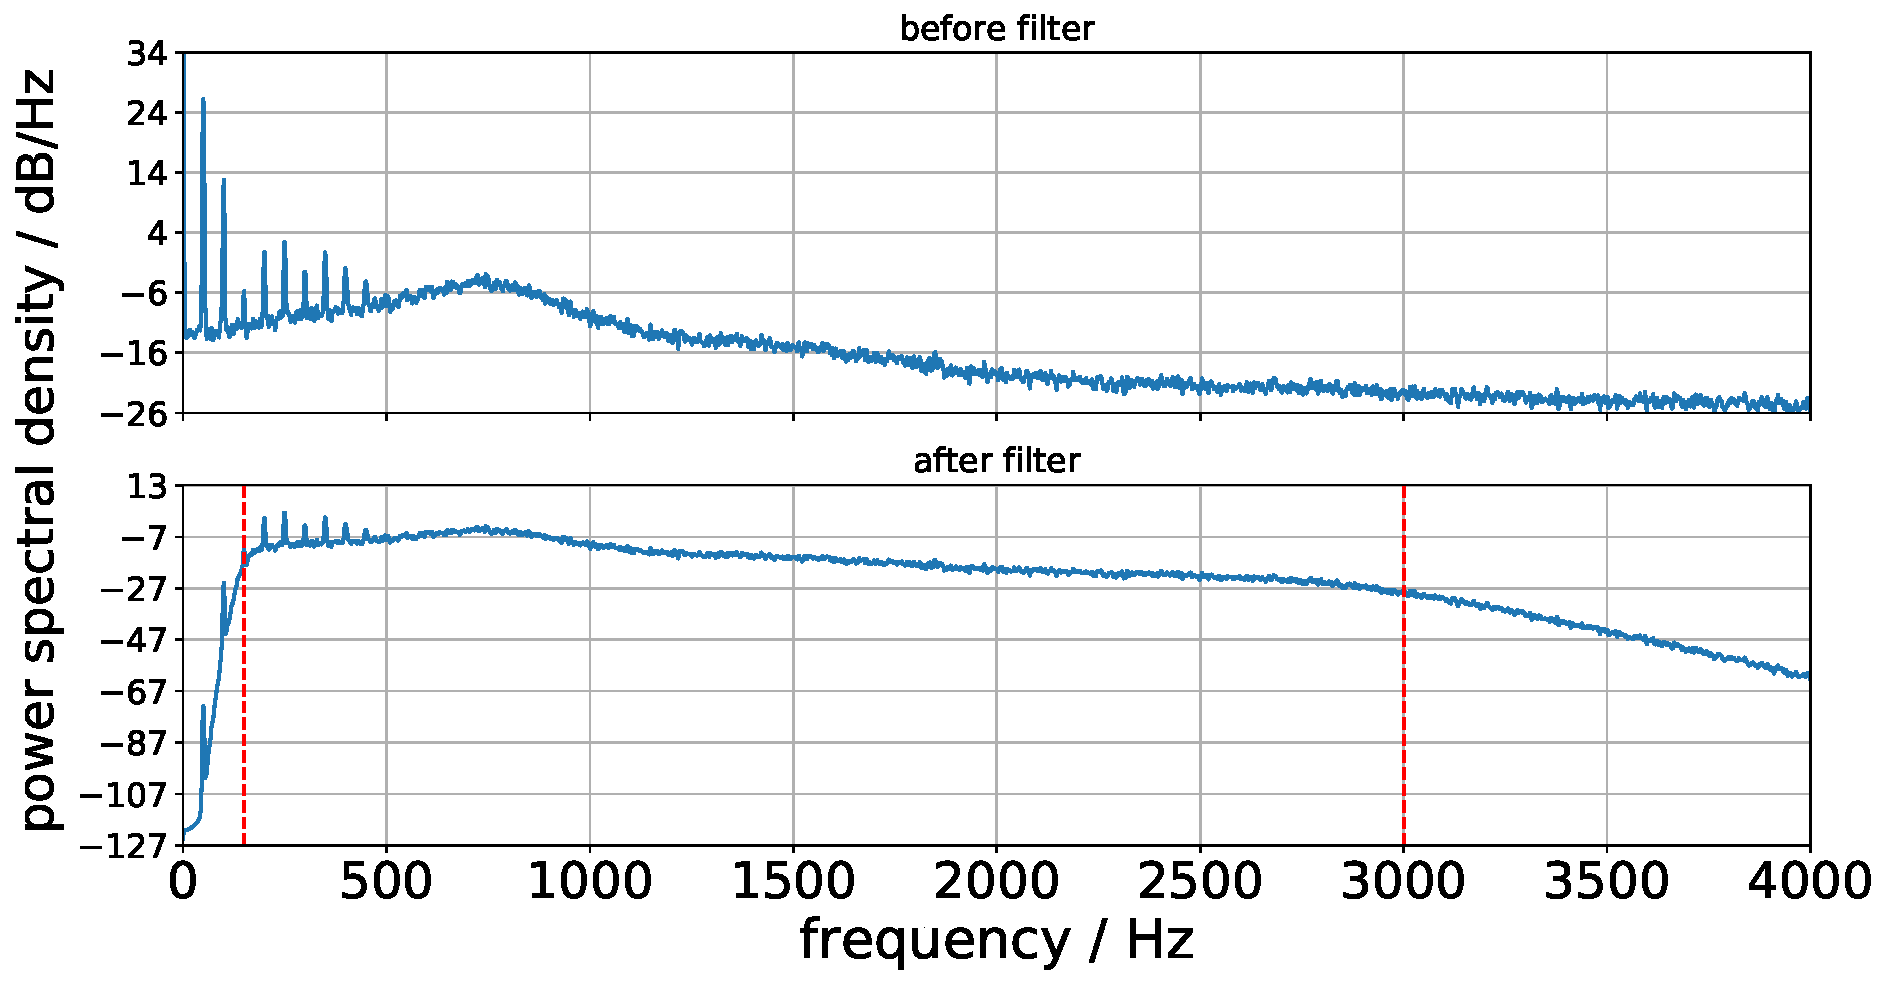
\includegraphics[width=.49\textwidth]{figures/psd_butterworth_14_6.pdf}
	\caption{\label{fig:psd_noise}
Power spectral density (PSD) of background noise (top) from the optical microphone (with the speaker off), and the PSD after applying a Butterworth bandpass filter (bottom) between the two frequencies marked with red, dashed lines. 
We see strong power from the $50\,{\rm Hz}$ mains hum and its harmonics (most likely from the photodiode circuit and the room’s lighting and cooling). Otherwise the PSD is fairly white. 
After filtering we see strong attenuation of all frequencies outside the band, but little change to the harmonics within the band.
}
\end{figure}


\subsection{A hierarchy of filters}
\label{sec:filters}

Here, we describe several filters used to remove the $50\,{\rm Hz}$ mains hum and its harmonics, but also to ultimately improve the speech intelligibility of the recording (to be able to understand the words). We start with some naive approaches and then move to traditional signal processing filters like band-passing and cascaded notches. We finish by combining these with advanced statistical techniques like a Wiener filter and the logMMSE estimator. As an illustrative example, we test all of these filters on the same $1\,{\rm s}$ long speech recording.

\begin{figure*}
	\begin{center}
    %% trim order is <left> <lower> <right> <upper>
	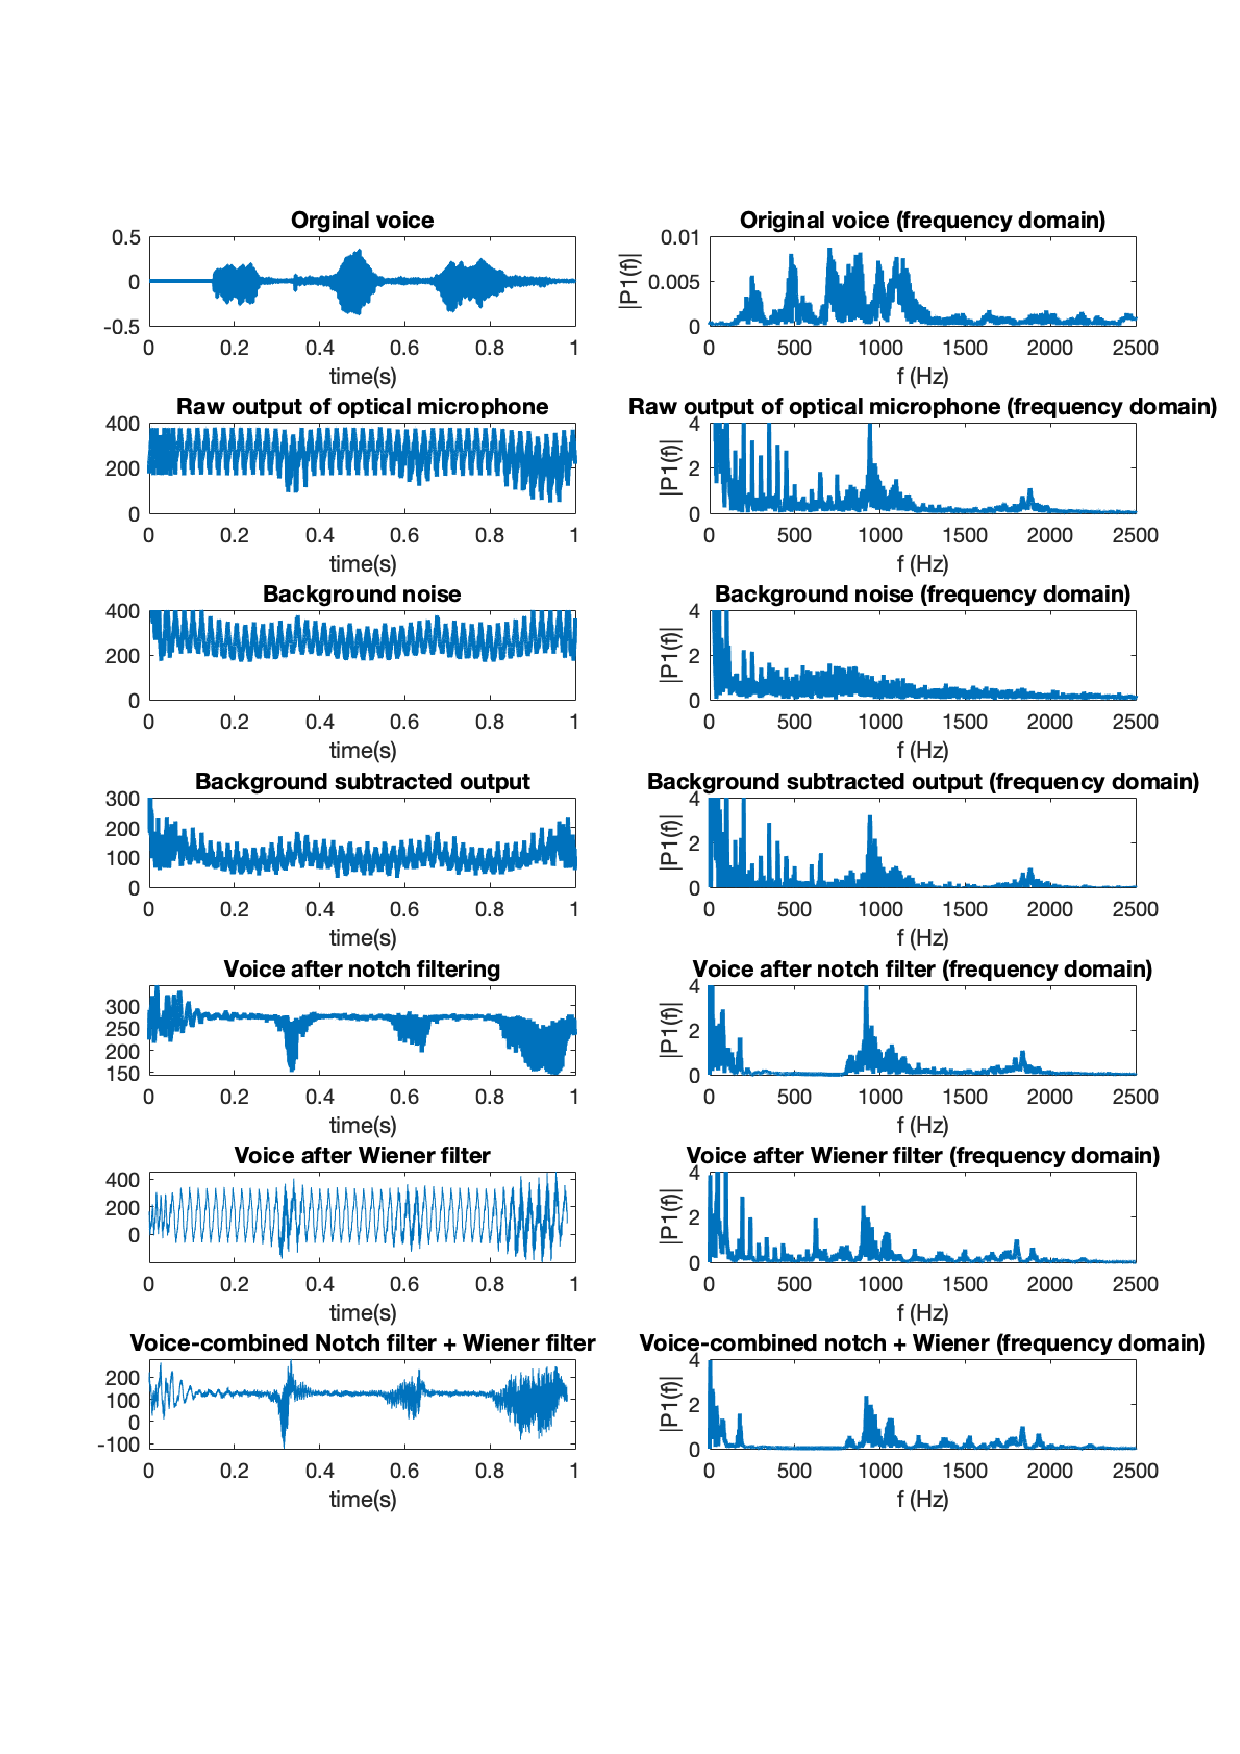
\includegraphics[width=\textwidth,trim={1cm 4.5cm 0.4cm 3.5cm},clip]{figures/notch_and_wiener_superplot_v2.pdf}
	\end{center}
	\caption{\label{fig:BackgroundNotchWienerCombined}
	Time series (left column) and frequency spectrum (right column) results for the background subtraction, notch, and Wiener filters.
	The first and second rows show the original speech recording and raw output from the optical microphone respectively. 
    The third row shows a background noise recording from the optical microphone when no audio signal is played. 
    The fourth row shows the result of subtracting the background noise spectrum in the third row from the recording in the second row. 
	%The second row shows the raw output from the optical microphone.
	%The third row shows the naive technique of subtracting off the noise spectrum from the recorded spectrum.
	The fifth, sixth, and seventh rows show the results of applying the notch filter, the Wiener filter, and both combined, respectively.
	}
\end{figure*}


%\begin{figure*}
%\begin{center}
%% trim order is <left> <lower> <right> <upper>
%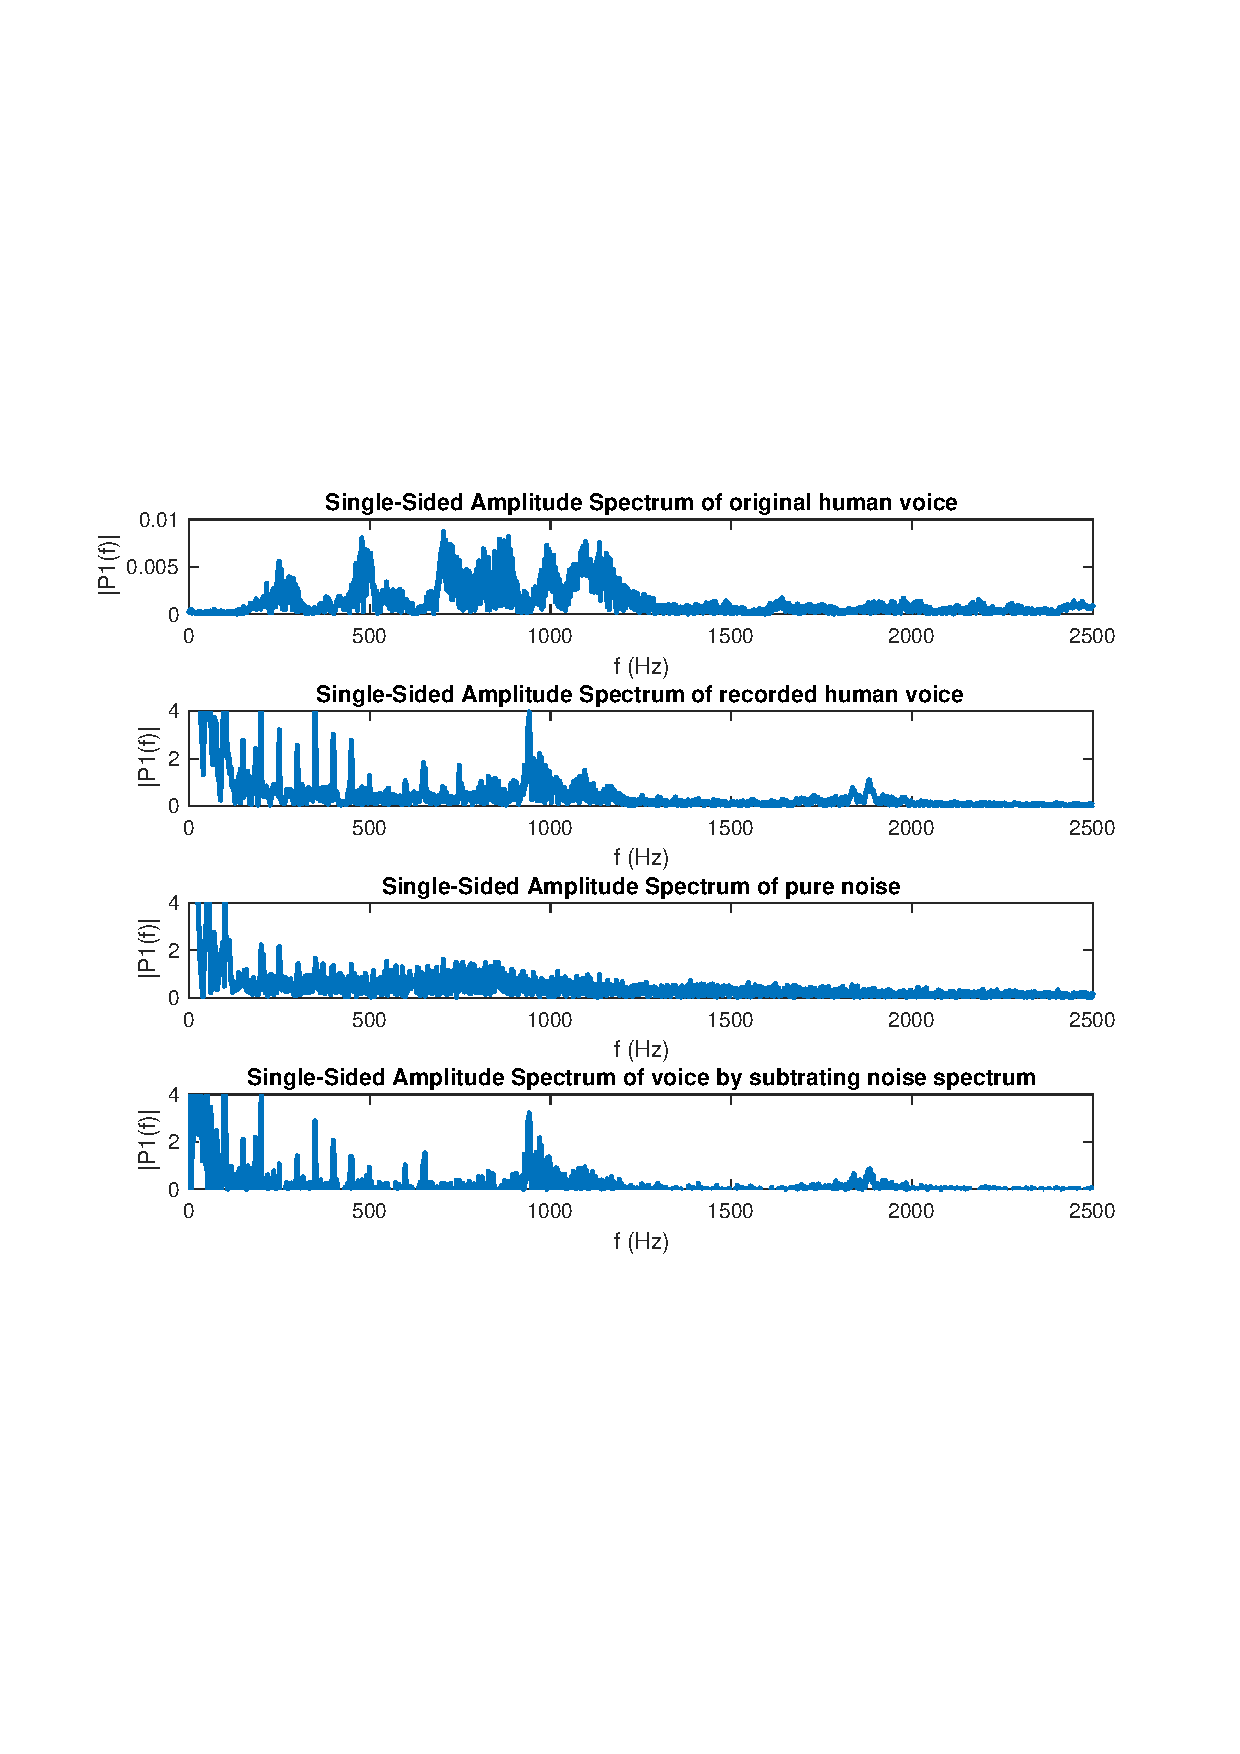
\includegraphics[width=\textwidth,trim={1cm 8.5cm 1cm 8cm},clip]{figures/freqSpectrumOriginalNoiseSubtracted.pdf}
%\end{center}
%\caption{\label{fig:noiseSubtract}
%Frequency spectrum of a $1\,{\rm s}$ signal before the use of filters. 
%The first panel shows the original frequency spectrum of the human voice recording (saying ``A cathode ...''). 
%The second panel shows the spectrum recorded after the signal passes through the optical microphone (sampled at $16\,000\,{\rm Hz}$).
%The third panel shows a noise-only recording from the optical microphone when no audio signal is being played. 
%The fourth panel shows the result of subtracting the noise-only spectrum in the third panel from the recording in the second panel. 
%We see no obvious improvement from this method. 
%}
%\end{figure*}

Results for a selection of filters are collated in Fig.~\ref{fig:BackgroundNotchWienerCombined} where the left and right columns show timeseries and Fourier spectrum results respectively. 
The first and second rows of Fig.~\ref{fig:BackgroundNotchWienerCombined} shows the source signal and the raw optical microphone recording respectively. 
The third row shows a background spectrum of the optical microphone, as shown previously in the top panel Fig.~\ref{fig:psd_noise}.

%The Fourier spectrum of the source signal is shown in the first panel of Fig.~\ref{fig:BackgroundNotchWienerCombined}. The second panel shows the spectrum of the raw optical microphone recording of the signal. The third panel of Fig.~\ref{fig:noiseSubtract} shows a background spectrum of the optical microphone, as shown previously in the top panel Fig.~\ref{fig:psd_noise}.

Given that we have access to the background noise spectrum, an intuitive way to remove noise is via subtracting the noise spectrum from the recorded spectrum. 
The fourth panel of Fig.~\ref{fig:BackgroundNotchWienerCombined} shows the spectrum obtained after subtracting the background noise spectrum. 
We see no obvious improvement, which may be attributed to a time-variant noise spectrum the cause of which is unidentified. %Why the noise sources are time-varying is a fact yet to be determined.


Beyond this na\"{i}ve approach, we apply a range of filters to the data.
In signals processing, the ideal filter would be one that:
%\begin{itemize}
i) completely attenuates the undesired parts of the spectrum, 
ii) does not change the rest of the spectrum, and 
iii) smoothly transitions between these regions, as to not damage the time domain signal when seen under convolution. 
%\end{itemize}
However, these three conditions cannot all hold at once and any filter must compromise between them. 



\subsubsection{Comb filter}

Simply zeroing the frequency bins corresponding to the harmonics of the $50\,{\rm Hz}$ mains signal is unsuccessful. This effectively multiplies the spectrum by a rectangular comb filter. It does remove the mains harmonics, but audibly ruins the rest of the signal due to lack of smoothness. This is because applying a filter in frequency space is equivalent to convolving the signal with the inverse Fourier transform of that filter. The inverse Fourier transform of a rectangular comb filter (a set of boxcars) is some combination of sinc functions, which significantly corrupt the signal. 
See also Section~\ref{sec:notch} where we explore a notch filter. 

%A smoother comb filter significantly attenuates the spectrum between each harmonic so that the signal is no longer audible. 
% \jam{[re:comb filters. When I tried to comb filter it either was too sharp and so jumbled the whole signal in convolution. Or if smooth attenuated the signal away into noise. At least, that's what I remember. Changrong has a comb filter section anyway so I am happy dropping my unsuccessful attempts.]}

\subsubsection{High-pass filter}

A high-pass filter smoothly attenuates frequencies below some cut-off frequency. Applying a high-pass filter, with a cut-off frequency around $150\,{\rm Hz}$, to the signal spectrum works well at removing the $50\,{\rm Hz}$ and $100\,{\rm Hz}$ harmonics. However, the mains harmonics above $100\,{\rm Hz}$ remain. Using a high-pass filter with a higher cut-off can be used to mitigate this issue. However, it makes the played-back signal unrecognisable as the region above $100\,{\rm Hz}$ carries a lot of the fundamental frequencies of speech and music~\cite{speech_intelligibility}.
Often in speech processing the logarithm of the signal is taken since the amplitude information seems to be more important to intelligibility than the phase information. However, applying a high-pass filter to the logarithm of the signal spectrum does not significantly improve on the above simple high-pass filter.

%We also tried applying a high-pass filter to the logarithm of the signal spectrum and then exponentiating back, but this didn’t significantly improve on the above simple high-pass

\subsubsection{Butterworth band-pass filter}

\begin{figure}
	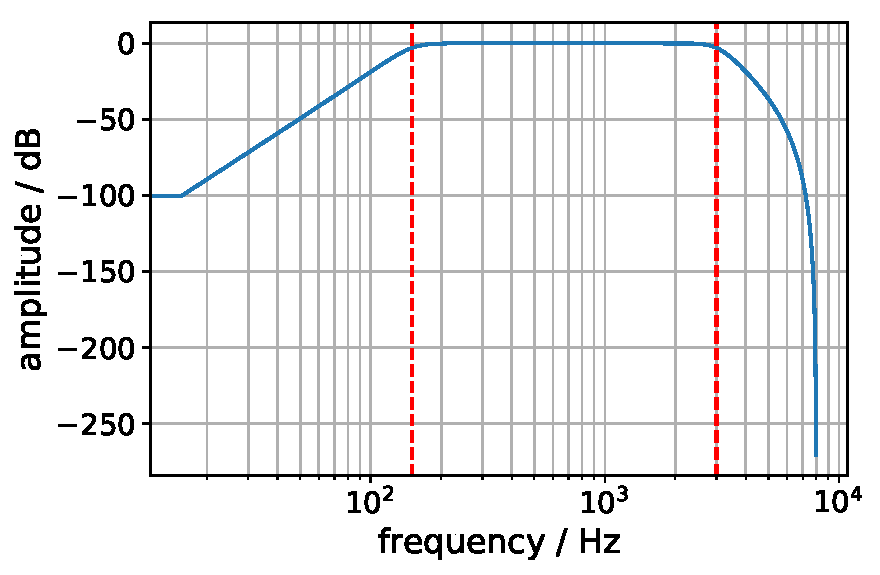
\includegraphics[width=0.49\textwidth]{figures/butterworth_150_3000.pdf}
	\caption{Butterworth bandpass filter frequency response, any amplitude beyond $-3\,{\rm dB}$ is significant attenuation (half power). The red, dashed vertical lines show the band limits of $150\,{\rm Hz}$ and $3\,{\rm kHz}$. Note the flat response within the band.}
	\label{fig:butterworth}
\end{figure}

A band-pass filter combines a high-pass filter and a low-pass filter to smoothly attenuate frequencies outside of some band. A Butterworth band-pass filter is just a particular choice of the frequency response (an attenuation at each frequency) as to be `maximally flat' within the pass-band region. The Butterworth low-pass component is given by Eqn.~\ref{eq:butterworth} and is combined with a similar high-pass filter to form the band-pass filter.

\begin{equation}
\label{eq:butterworth}
H(\omega) = \left[1+\varepsilon^2 \left( \frac{f}{f_c} \right)^{2n}\right]^{-1/2},
\end{equation}
% commenting to send to co-authors
%\jam{[Andrew wanted a quantitative comment about what the Butterworth does to the PSD, what do I use?]}

In the above expression, $f_c$ represents the cut-off frequency of the low-pass Butterworth filter, $\varepsilon$ represents the gain, and $n$ is the order of the filter which determines how quickly the response rolls off past the cut-off frequency. Fig.~\ref{fig:butterworth} shows the frequency response of the filter used here, a fifth order ($n = 5$) Butterworth filter with a pass-band of $(150\,{\rm Hz}$, $3\,{\rm kHz})$. This high frequency cut-off is chosen since the frequencies important for speech generally lie below $2\,{\rm kHz}$~\cite{speech_intelligibility}.

The effect of applying this filter to the background noise PSD can be seen in the bottom panel of Fig.~\ref{fig:psd_noise}. The Butterworth band-pass filter reduces the amplitude of mains harmonics below $150\,{\rm Hz}$ and suppresses unrelated noise sources above $3\,{\rm kHz}$. However, it does not address the issue of mains harmonics above $150\,{\rm Hz}$ (i.e., in the pass-band). In the following section, we experiment with a cascade notch filter to address this.



\subsubsection{Cascade notch filter}
\label{sec:notch}
\begin{figure*}
\begin{center}
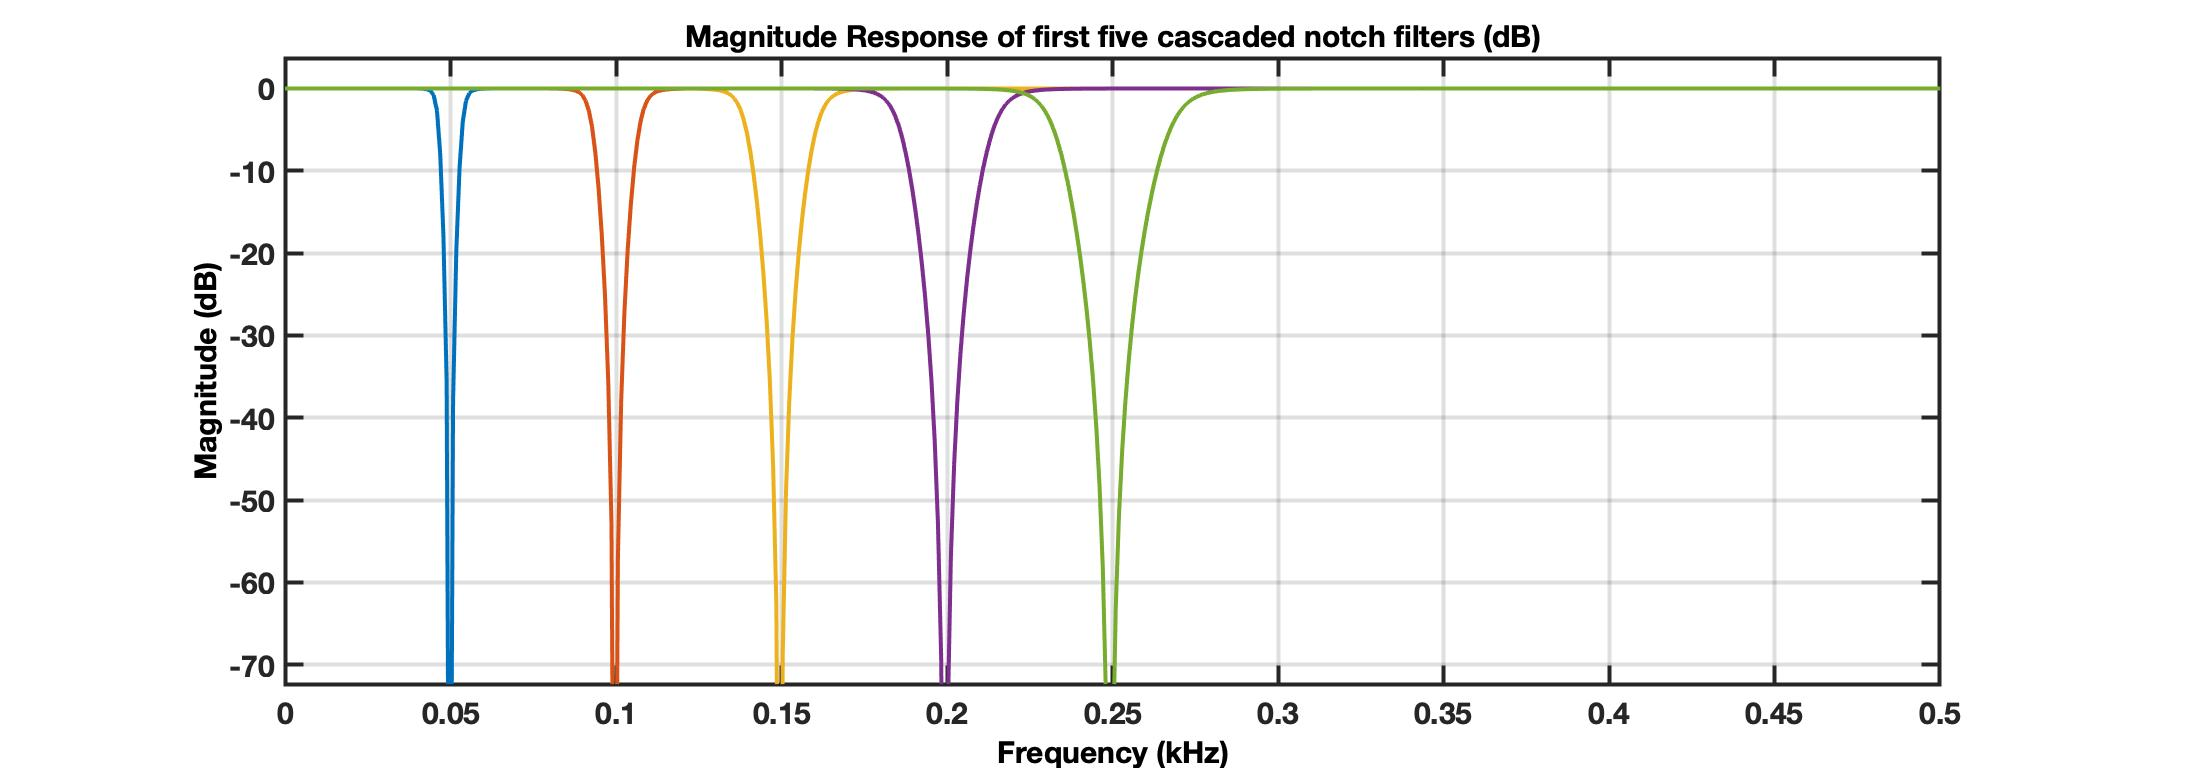
\includegraphics[width=.9\textwidth]{figures/notch_filter_response.jpg}
\end{center}
\caption{\label{fig:notchMagResponse}
Magnitude response for the first five notches of the $15$ cascaded notch filter described by Eqns.~\ref{eqn:notch} and ~\ref{eqn:notch15}. 
}
\end{figure*}

One method to remove mains noise and its harmonics is to use a sequence of notch filters centred at each of the frequency bins we want to remove. This sequence is known as a cascade of notches. Here the notches are smooth in comparison to the naive zeroing of each frequency (which looks like a rectangular comb). The complex frequency response of a typical infinite impulse response (IIR) notch filter can be written as \citep{10.5555/541204}
\begin{equation}
    \label{eqn:notch}
    H(z)=\frac{1+\alpha}{2}\frac{1-2\beta z^{-1}+z^{-2}}{1-\beta(1+\alpha)z^{-1}+\alpha z^{-2}}
\end{equation}
Where $z$ is the complex frequency and $\alpha$ and $\beta$ are parameters that control the filter. $w_0=\cos^{-1}(\beta)$ is the frequency that is completely attenuated (zeroed) at the centre of the notch and $B_w=\cos^{-1}[2\alpha/(1+\alpha^2)]$ is the bandwidth of the notch (which reflects how quickly the response changes around the notched frequency).
We find that a sequence of $15$ notches works well here, with the $k^\mathrm{th}$ notch centred on the $k^\mathrm{th}$ harmonic of the $50\,{\rm Hz}$ mains signal, where $k=0,2,\dots,14$. When then choose the bandwidth and order (here equal to six) of each notch to avoid disturbing useful signals while still allowing for uncertainty in the location of each harmonic of the mains signal. The response of this cascaded notch filter $H(z)$ is the product of the responses of each of the individual $H_k(z)$ notches,
\begin{equation}
    \label{eqn:notch15}
    H(z) = \prod_{k=0}^{14} H_k(z).
\end{equation}

We use the built-in MATLAB filter design toolbox in this work. 
The amplitude response of the first five notch filters is shown in Fig.~\ref{fig:notchMagResponse}. 
The time series and spectrum obtained after applying the cascade notch filter to the speech recording are shown in the fifth row of Fig.~\ref{fig:BackgroundNotchWienerCombined}.
We see that the mains harmonics are significantly attenuated in comparison background subtracted results shown in the fourth row of Fig.~\ref{fig:BackgroundNotchWienerCombined}.

Although the notch filter removes much of the mains hum sound, the filtered recording is not intelligible. Qualitatively it sounds more like a drum than a human voice. Evidently, this is due to loss of voice information under the filter.

% This effect will become more severe if the original human spectrum overlaps with the hum spectrum by a large amount.
To overcome this, we turn to more advanced techniques starting with the Wiener filter. Instead of just passively filtering different frequencies, this statistical technique optimises an estimate of the original signal. 
% By purely minimizing the "distance" between estimated signal (filtered human voice) and observed signal (original human voice), we hope that we keep signal part undisturbed while filtering out noise. 



% \begin{figure*}
% \begin{center}
% 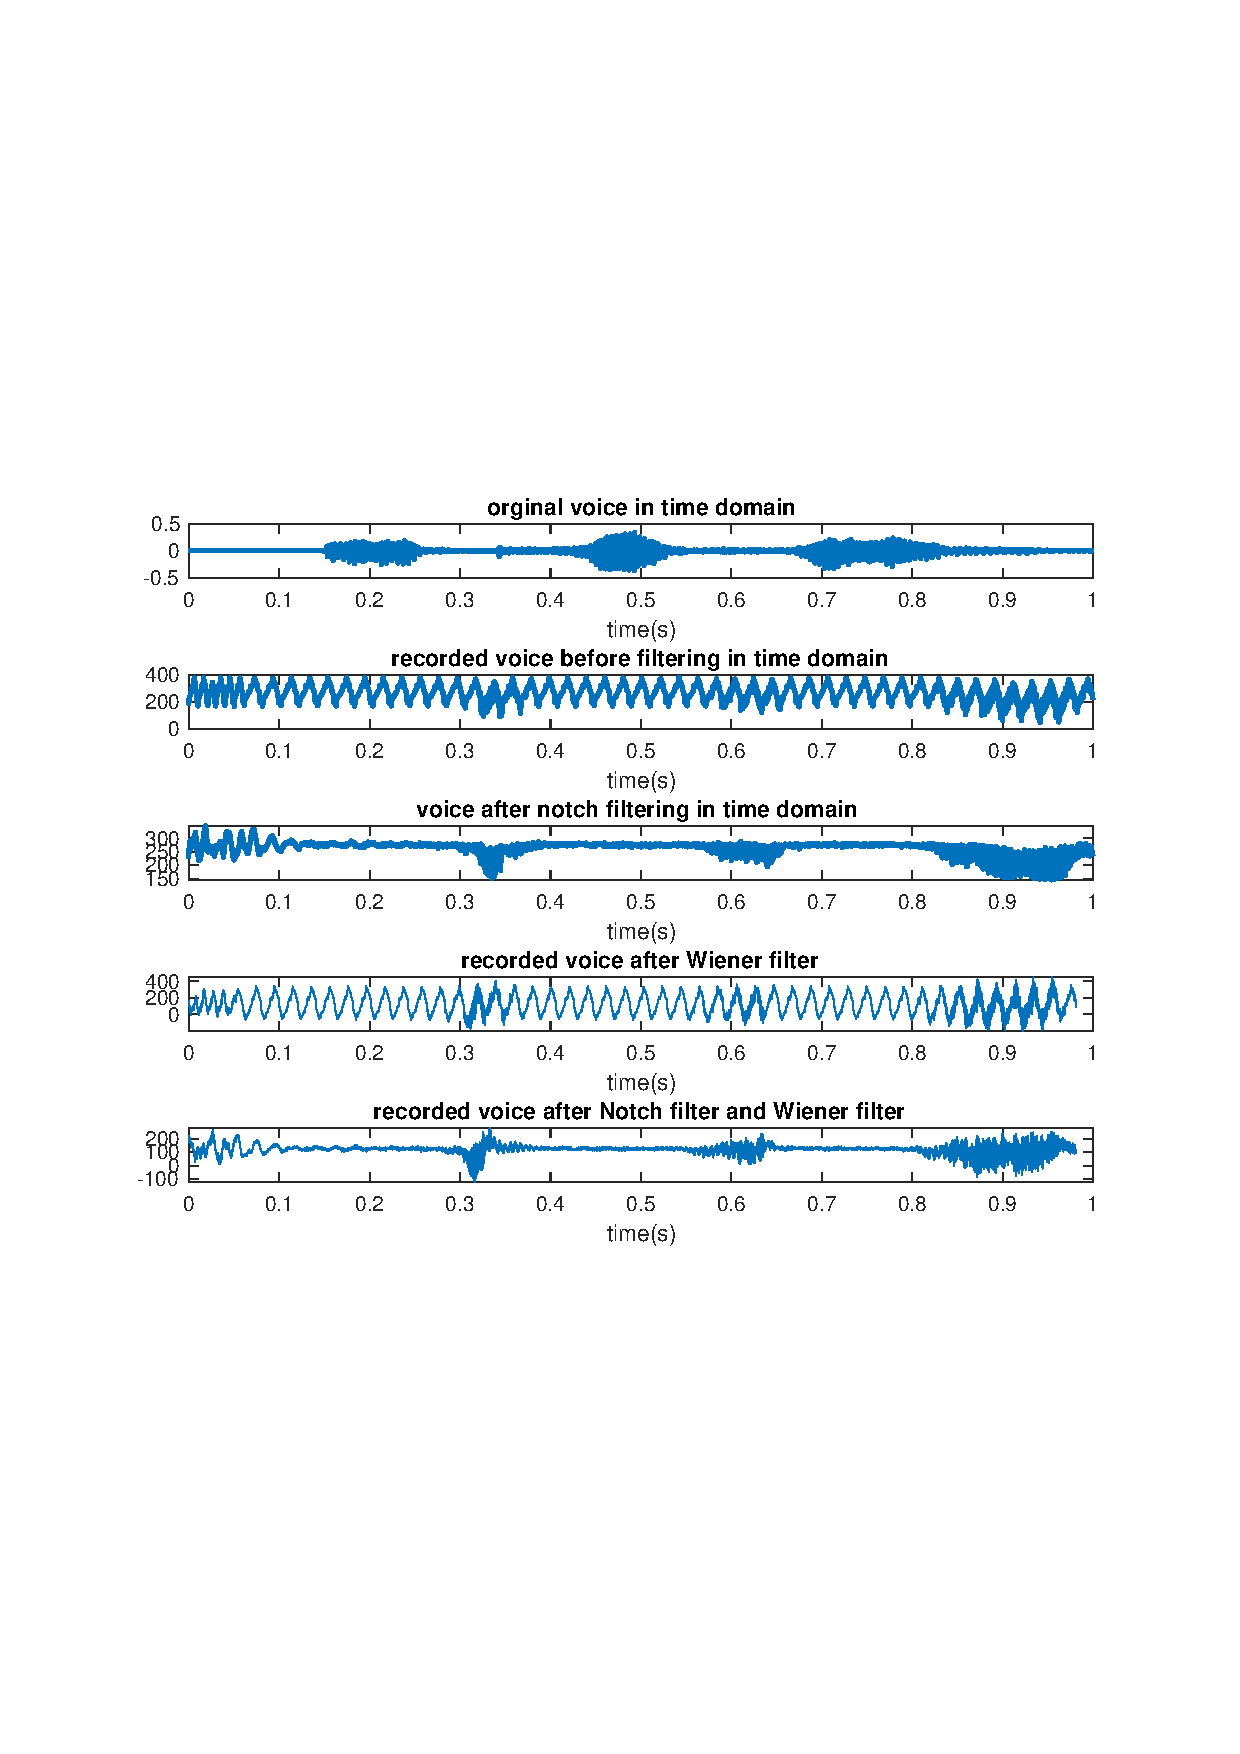
\includegraphics[width=\textwidth,trim={1cm 8.2cm 1 8.3cm},clip]{figures/timeSeriesNotchWiener.pdf}
% \end{center}
% \caption{\label{fig:timeNotchWiener}
% Timeseries results for the notch and Wiener filters. 
% The first panel shows the original speech recording which was played from the speaker. 
% The second panel shows the data from the optical microphone before any filters are applied. 
% The third and fourth panels show results after applying the notch and Wiener filter respectively. 
% Finally, the fifth panel shows the result of applying both the notch and Wiener filter. 
% }
% \end{figure*}

% \begin{figure*}
% \begin{center}
% 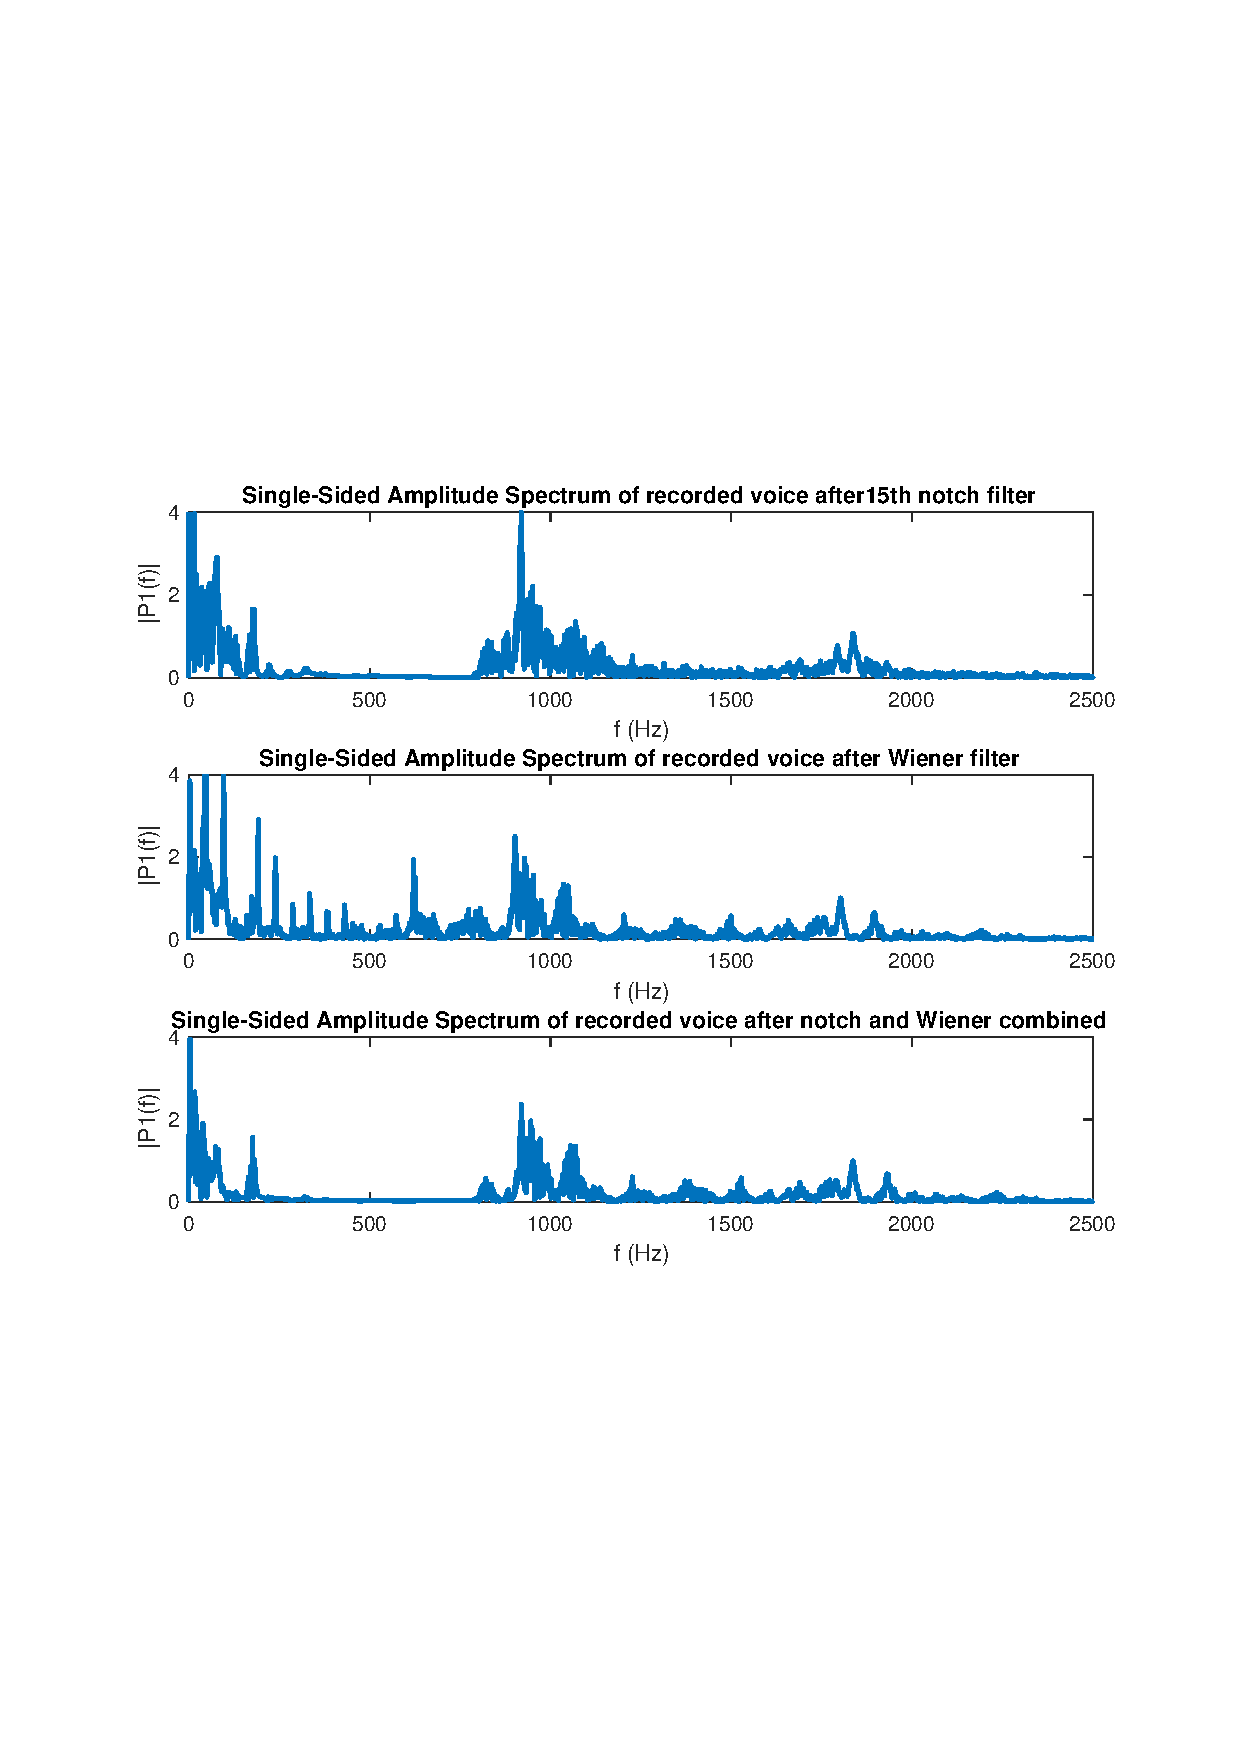
\includegraphics[width=\textwidth,trim={0cm 8.2cm 0cm 8cm},clip]{figures/freqNotchWiener.pdf}
% \end{center}
% \caption{\label{fig:freqNotchWiener}
% Frequency spectrum results for the notch and Wiener filters. 
% The first and second panels show the results of applying the notch and Wiener filter respectively.
% The third panel shows the spectrum after applying both the notch and Wiener filters. 
% The first, second, and third panels show the spectrum of the timeseries show in the third, fourth, and fifth panels of Fig.~\ref{fig:timeNotchWiener} respectively. 
% }
% \end{figure*}

%A notch filter attenuates signals in specific frequency bands. 
%We apply a $15$ cascaded notched filter to remove the mains noise and its harmonics up to $750\,{\rm Hz}$. 
%\han{should we include here a mathematical description of the $15$ cascade notch filter?}
%\jam{[Yes, I have no idea what a cascaded notched filter is and I'm an author!]}



\subsubsection{Wiener Filter}

A Wiener filter is an advanced statistical technique that estimates the injected signal given prior information about the injected spectrum and the reference spectrum of the background noise. Let the observed noisy speech signal sequence be given as $\mathbf{x}=\{x(0),\dots, x(N-1)\}$, where $N$ is the length of the data sequence. It is the sum of the original injected signal $\mathbf{s}=\{s(0),\dots,s(N-1)\}$, and the noise sequence $\mathbf{w}=\{w(0),\dots,w(N-1)\}$, 
\begin{equation}
    \mathbf{x}=\mathbf{s}+\mathbf{w}\,.
\end{equation}
Given the observed data $\textbf{x}$, our goal is to make an estimate $\hat{\textbf{s}}$ of the original signal $\textbf{s}$ such that we minimise the Bayesian mean square error (BMSE) between the two, defined as 
\begin{equation}
\label{eq:BMSE}
\text{BMSE}(\hat{\textbf{s}})=E[(\textbf{s}-\hat{\textbf{s}})^2]\,,
\end{equation}


If we assume that: i) $\textbf{x}$ is \emph{wide sense stationary}~\footnote{ A random process $\{x(t)\}$ is wide sense stationary if, for all $t_1,t_2 \in R$, (1) its mean is time invariant, i.e., $\mu_x(t_1)=\mu_x(t_2)=\text{constant}$; and (2) the autocorrelation depends only on the time difference, i.e., $R_x(t_1,t_2)=R_x(\tau),\tau=t_1-t_2$.} with zero mean; ii) the signal $\textbf{s}$ has a mean of zero; and iii) the noise $\textbf{w}$ is uncorrelated with the signal $\textbf{s}$, we can further express $\hat{\textbf{s}}$ to be a linear combination of present and past observed data
\begin{equation}
\hat{{s}}[n]=\sum_{k=0}^{n}h[k]x[n-k]\,,
\end{equation}
where $\textbf{h}=\{h(0),\dots h(n)\}$ represents the coefficients of an $n$th order Wiener filter.
% What this sentence is trying to convey is not clear to me
%% just trying to say that we can make the assumptions that we do because the Wiener filter appears to work well under them - J
%These assumptions are to be justified by the efficacy of the Wiener filter.
%Given the observation data $\mathbf{x}$, our goal is to estimate $\mathbf{s}$ so that the error between $\mathbf{x}$ and the estimate ${\hat{\mathbf{s}}}$ is minimized in the mean square sense,
%\begin{equation}
%    \hat{\mathbf{s}}=\mathop{\arg\min}_{\textbf{s}}||\mathbf{x}-\mathbf{s}||_2^2\,. 
%\end{equation}
%Assuming that $\textbf{x}$ is wide-sense stationary~\footnote{
%A random process $\{x(t)\}$ is wide sense stationary (WSS) if for all
%$t_1,t_2 \in R$, it satisfies (1) mean is time invariant, i.e.,
%$\mu_x(t_1)=\mu_x(t_2)=\text{constant}$; (2) autocorrelation depends
%only on time difference, i.e., $R_x(t_1,t_2)=R_x(\tau),\tau=t_1-t_2$.}
%and that $\textbf{w}$ is stationary and uncorrelated with the signal, we represent the $n$th order Wiener filter by its coefficients $\textbf{h}=\{h(0),\dots(n)\}$. 
The famous Wiener-Hopf equation~\citep{noble1959methods} allows us to determine $\textbf{h}$, as\begin{equation}
\label{eqn:wiener-hopf}
\begin{bmatrix}  
r_{xx}[0]&r_{xx}[1]&\dots& r_{xx}[n]\\
r_{xx}[1]&r_{xx}[0]&\dots &r_{xx}[n-1]\\
\vdots&\vdots&\ddots&\vdots\\
r_{xx}[n]&r_{xx}[n-1]&\dots &r_{xx}[0]
\end{bmatrix}
\begin{bmatrix}
h[0]\\
h[1]\\
\vdots\\
h[n]
\end{bmatrix}=
\begin{bmatrix}
r_{ss}[0]\\
r_{ss}[1]\\
\vdots\\
r_{ss}[n]
\end{bmatrix}\,,
\end{equation}
where $r_{xx}$ and $r_{ss}$ are the auto-correlation functions of $\mathbf{x}$ and $\mathbf{s}$ between timestep $i$ and $i+n$, 
%\begin{equation*}
%\left\{ 
\begin{eqnarray} 
r_{xx}[n] &~=~& E[x(i)~x(i+n)] \,,\\
r_{ss}[n] &~=~& E[s(i)~s(i+n)] \,.
%r_{xx}[n] &=& E[x(i)\, &x(i+n)] \\ 
%r_{ss}[n] &=& E[s(i)\, &s(i+n)] 
\end{eqnarray} 
%\right\}  
%\end{equation*}
%where $r_{xx}$ and $r_{ss}$ is the auto-correlation function of $x$ and $s$.


%As an instructive aside, i
If we let the Wiener filter be non-causal (i.e. we estimate the current signal based on both past \emph{and future} observations), then we can represent Eqn.~\ref{eqn:wiener-hopf} in the frequency domain as
\begin{equation}
\label{eqn:wiener}
    H(f)=\frac{P_{ss}(f)}{P_{xx}(f)}=\frac{P_{ss}(f)}{P_{ss}(f)+P_{ww}(f)}
\end{equation}
where $P_{xx}(f), P_{ss}(f), P_{ww}(f)$ are the spectra of the observed noisy data, the injected signal, and the background noise, respectively. Intuitively, from Eqn.~\ref{eqn:wiener}, we can see that the non-causal Wiener filter amplifies the input signal where the signal to noise ratio (SNR) is high, and attenuates the signal where the SNR is low. The causal Wiener filter (that only makes estimates based on past observations) is similar. More detailed analysis of both kinds of Wiener filters can be found in Ref.~\citep{10.5555/151045}.
% That this filter is non-causal makes it unsuitable for real time signal processing 

%In this work, we construct a causal Wiener filter based on Eqn.~\ref{eqn:wiener-hopf}, and set the length of the filter to $n=100$. 
%A larger $n$ provides more smoothing of the input signal, however requires more computational memory. 
%The choice of $n=100$ is a reasonable selection to balance smoothing and efficiency. 

In this work, we construct a higher-order causal Wiener filter based on Eqn.~\ref{eqn:wiener-hopf}. A higher order Wiener filter provides greater smoothing of the input signal but also increases the computational memory required. For this work, we choose a Wiener filter of order $n=100$ as it provides a reasonable balance between smoothing and efficiency. The time series and frequency spectrum after applying the Wiener filter are shown in the sixth row of Fig.~\ref{fig:BackgroundNotchWienerCombined}.
We see a significant improvement in the time series of the recovered signal, however a strong noise hum persists, audibly. 
%The Wiener filter produces an estimated signal $\hat{x}$ using linear time-invariant filtering. 
%It minimizes the mean square error $\mathbb{E}[(\hat{x}-x)^2]$ between $\hat{x}$ and the actual signal $x$~\citep{verhoeven2009robust}.
%\han{should we add more details here too?} \jam{[seconded]}
%The timeseries and frequency spectrum results of the Wiener filter are shown in the fourth panel of Fig.~\ref{fig:timeNotchWiener} and the second panel of Fig.~\ref{fig:freqNotchWiener} respectively. 
%The timeseries is visibly cleaner, however there is a strong noise hum. 


\subsubsection{Combined notch and Wiener filter}

Here we experiment with applying a combination of the cascaded notch and the Wiener filter to the recorded speech signal. 


The Wiener filter makes use of statistical information from the speech data and noise. It amplifies the part of the signal with high SNR, while suppressing the parts with low SNR. It is implemented in the form of a finite response filter, which ensures linear phase response and stability (both desirable), but at the cost of high orders computationally. By comparison, the notch filter is based on directly removing the unwanted frequency components. It is implemented in the form of an infinite impulse response filter. Although it significantly decreases the order of the overall filter, it unavoidably introduces nonlinear phase and instability. 


By combining the notch and Wiener filter, we can trade off between the two and achieve an overall better performance, as can be seen in the bottom row of Fig.~\ref{fig:BackgroundNotchWienerCombined}..
The filtered voice after the combined notch and Wiener filter is enhanced compared to either alone. The mains noise is all but removed and more voice information is retained. However, the recovered voice still sounds muffled and is not understandable.


%The combination of the notch filter and the Wiener filter produces a cleaner signal than either individually. 
%The time series and spectrum results are shown in the final panels of Figs.~\ref{fig:timeNotchWiener} and ~\ref{fig:freqNotchWiener} respectively.

%The ideal filter would be one that i) completely attenuates the undesired parts of the spectrum, ii) does not change the rest of the spectrum, and iii) has smooth edges so as to not damage the signal after convolution. 
%These three conditions are contradictory and any filter must compromise between them. 
%The above simple filters fail one or more of i)--iii). 
%The Butterworth filter performs the best as it is optimised to be `maximally flat' within the band region, prioritising the second condition.
%\han{see note from Andrew and ask James about this}




%\han{Is it worth also including some plots to show how the different filters perform? E.g. a PSD with comb filter, high pass filter, Butterworth filter?}

% Note that we also replicated the Viterbi algorithm results from before with the photodiode, but only with the mains hum removed and high-passing above 100Hz, else the algorithm never selected the signal. Except for being over audible frequencies, there isn’t much difference in the tracking once these filters are applied.


\subsubsection{logMMSE estimator}
\label{sec:logmmse}


\begin{figure*}
	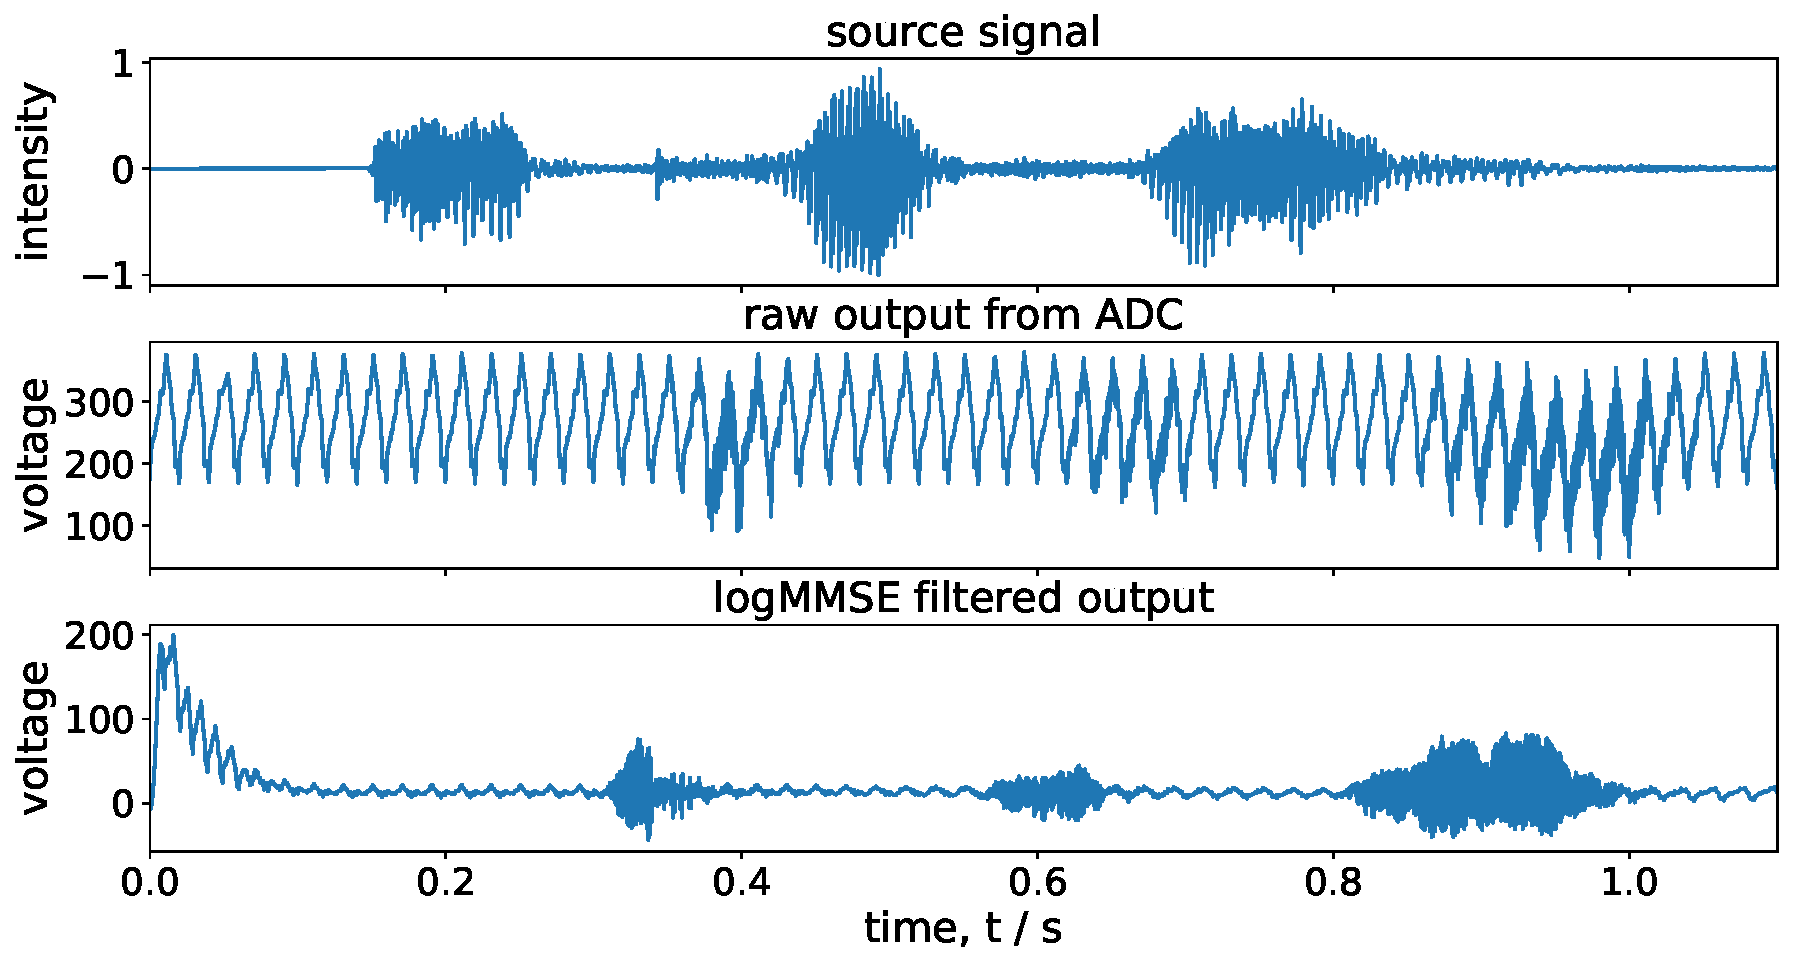
\includegraphics[width=\textwidth]{figures/combined_timeseries_melatos.pdf}
	\caption{Time series of an adult male voice (saying ``A cathode ...'') showing the source (top panel), the optical microphone recording (middle panel), and the recording after filtering with the logMMSE estimator (bottom panel). One second of the one minute recording is shown. The rise at the start of the bottom panel is expected when filtering a signal of finite duration.}
	\label{fig:logMMSE_timeseries}
\end{figure*}

\begin{figure*}
	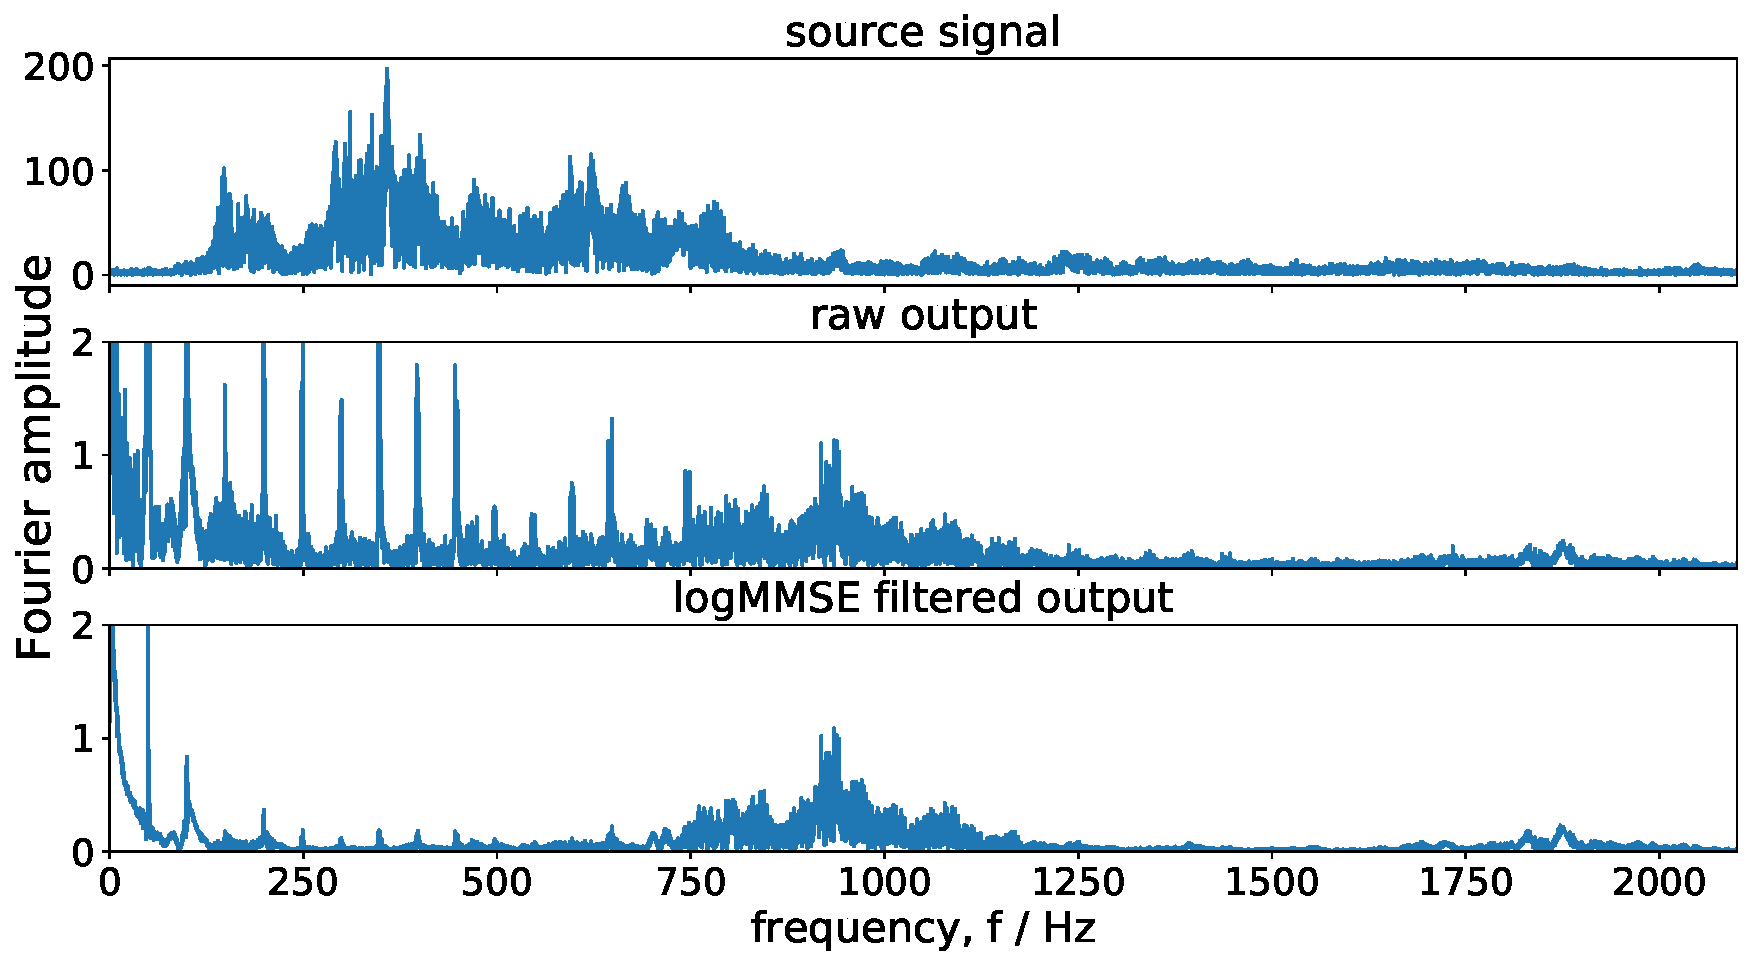
\includegraphics[width=\textwidth]{figures/combined_spectrum_melatos.pdf}
	\caption{Spectrum of optical microphone recording of the same adult male voice in Fig.~\ref{fig:logMMSE_timeseries} showing the source (top panel), the optical microphone recording (middle panel), and the recording after filtering with the logMMSE estimator (bottom panel). The spectrum shows only a detail of the total frequency domain (there is little activity at higher frequencies) and has truncated peaks at amplitude 2 which otherwise dominate the plot.}
	\label{fig:logMMSE_spectrum}
\end{figure*}


%probably a bit too causal language 
%What we’re attempting here is not new, 
Speech enhancement of noisy channels is a classic problem in signal processing. 
% shouldn't we make the citations consistent throughout? We don't mention author names up to this point and typically journals have a set style guide. - Hannah 
%To borrow from that field, Yi Hu and P.C. Loizon~\cite{SubjectiveComparison} compared $13$ speech enhancement methods and found the log minimum means-square error (logMMSE) estimator to be the best among them, qualitatively, at recovering speech. 
In Ref.~\cite{SubjectiveComparison} a comparison is made of $13$ speech enhancement methods, finding the log minimum means-square error (logMMSE) estimator to be the best, qualitatively, at recovering speech. 
This estimator is based on speech enhancement techniques discussed in Ref.~\cite{Ephraim1984SpeechEU_logMMSE} and minimises the mean square error (MSE) of the estimate from the injected signal, like the Wiener filter above, except that is measures the MSE between the logarithm of the Fourier amplitudes. This is motivated by the fact that the logarithm approximates the response of the human ear~\cite{SubjectiveComparison}. We apply an existing implementation of the logMMSE estimator (see Ref.~\cite{logmmse}) to the recorded signal.
%Hu~\&~Loizou~(2006)~\cite{SubjectiveComparison} compare 13 speech enhancement methods and find the best to be a log minimum mean-square error (log-MMSE) estimator. 
%This type of estimator is based on work Ephraim~\&~Malah~(1984)~\cite{Ephraim1984SpeechEU_logMMSE} into speech enhancement by minimising the mean square error (MSE) to the logarithm of the spectral (Fourier) amplitude.

%In this work we use an existing implementation~\cite{logmmse} of the logMMSE estimator. 
%Applying this estimator to the optical microphone output produced dramatically cleaner results. 
 



The results of the logMMSE estimator are shown in Figs.~\ref{fig:logMMSE_timeseries} and~\ref{fig:logMMSE_spectrum}. The top two panels of each figure show the original speech signal and anti-aliased reading from the optical microphone for ease of comparison. The third panel of Figs.~\ref{fig:logMMSE_timeseries} and~\ref{fig:logMMSE_spectrum} show the time series and corresponding spectral amplitude respectively after applying the logMMSE estimator. We see significant attenuation of the mains harmonics as well as a general smoothing of the spectrum. The logMMSE method indeed removes most of the background noise, but does not significantly enhance the speech as the voice sounds muffled and indistinct.
% suggest remove as it's just rephrasing what's already been said
%, with the words unable to be understood.


We find some improvement with music over speech. After applying the logMMSE estimator, simple chords and drums can be heard, however more composite sounds and complex melodies cannot be heard clearly. 
%Our observations suggest that this is especially true for instruments of certain timbres (harmonic profiles), in particular flutes and violins sometimes can’t be heard at all. 
Our observations suggest that this is especially true for certain instruments, in particular flutes and violins sometimes can’t be heard at all. 
This could be a perceptual effect or a frequency dependence somewhere in the optical microphone.
%, although the exact cause is yet to be determined.  - repetition
Speculating, perhaps the speaker-mirror coupling is stronger at low frequencies and thus instruments like electric bass and drums are louder in the results.


To address these problems, we need to determine whether the signals that are audibly missing (the diction in the speech and complex melodies in music) are indeed being transmitted through the optical microphone at all. 
%Or if instead they are present in the noisy data but we need better techniques to extract them. - should probably justify what you mean by better if you are going to say it here, but I think enough is discussed in section VI for it not to be necessary here - hannah 
To determine this requires a better understanding of the system as discussed in Section~\ref{sec:future_work}.



%Overall, we find that the intelligibility of speech remains low. 
%The played-back voice sounds mumbled and indistinct. 
%The estimator removes most of the background noise, but does not clarify the speech. 
%To address these problems with the recordings we need to determine whether the signals that are audibly missing (the diction in the speech and complex melodies in music) are indeed being transmitted through the optical microphone at all. 
%This requires a better understanding of the system.
% The fringe counting problem of the detector, wherein multiple fringes passing over the array in a single speaker deflection artificially raises the frequency, was noticeable in the speech recordings when compared to the source audio. However, upon comparing injected pure tones, the increase appears to be minimal and inconsistent, at around 5Hz maximum difference. An simple explanation is that the speaker deflections are small compared to manual pressing on the optical table.



\end{document}
